\section{Introduction}
\label{sec:intro}


\IEEEPARstart{R}{ecent} years have seen the remarkable progress of LLMs~\cite{zhao2023survey,chatgpt, openai2023gpt4, vicuna, llama}. 
By scaling up data size and model size, these LLMs raise extraordinary emergent abilities, typically including instruction following ~\cite{llama, peng2023instruction}, In-Context Learning (ICL) ~\cite{brown2020language}, and Chain of Thought (CoT) ~\cite{wei2022chain}. 
Although LLMs have demonstrated surprising zero/few-shot reasoning performance on most Natural Language Processing (NLP) tasks, they are inherently ``blind'' to vision since they can only understand discrete text. 
Concurrently, Large Vision Models (LVMs) can see clearly~\cite{sam, shen2023aligning, dino, dinov2}, but commonly lag in reasoning. 

In light of this complementarity, LLM and LVM run towards each other, leading to the new field of Multimodal Large Language Model (MLLM).
Formally, it refers to the LLM-based model with the ability to receive, reason, and output with multimodal information.
Prior to MLLM, there have been a lot of works devoted to multimodality, which can be divided into discriminative~\cite{clip,li2021align,chen2020uniter} and generative~\cite{wang2022ofa,cho2021unifying,wang2021simvlm} paradigms.
CLIP~\cite{clip}, as a representative of the former, projects visual and textual information into a unified representation space, building a bridge for downstream multimodal tasks. 
In contrast, OFA~\cite{wang2022ofa} is a representative of the latter, which unifies multimodal tasks in a sequence-to-sequence manner. 
MLLM can be classified as the latter according to the sequence operation, but it manifests two representative traits compared with the traditional counterparts: 
(1) MLLM is based on LLM with billion-scale parameters, which is not available in previous models.
(2) MLLM uses new training paradigms to unleash its full potential, such as using multimodal instruction tuning~\cite{wei2021finetuned,llava} to encourage the model to follow new instructions.
Armed with the two traits, MLLM exhibits new capabilities, such as writing website code based on images~\cite{minigpt-4}, understanding the deep meaning of a meme~\cite{mm-react}, and OCR-free math reasoning~\cite{palm-e}.

\begin{figure*}[t]
    \centering
    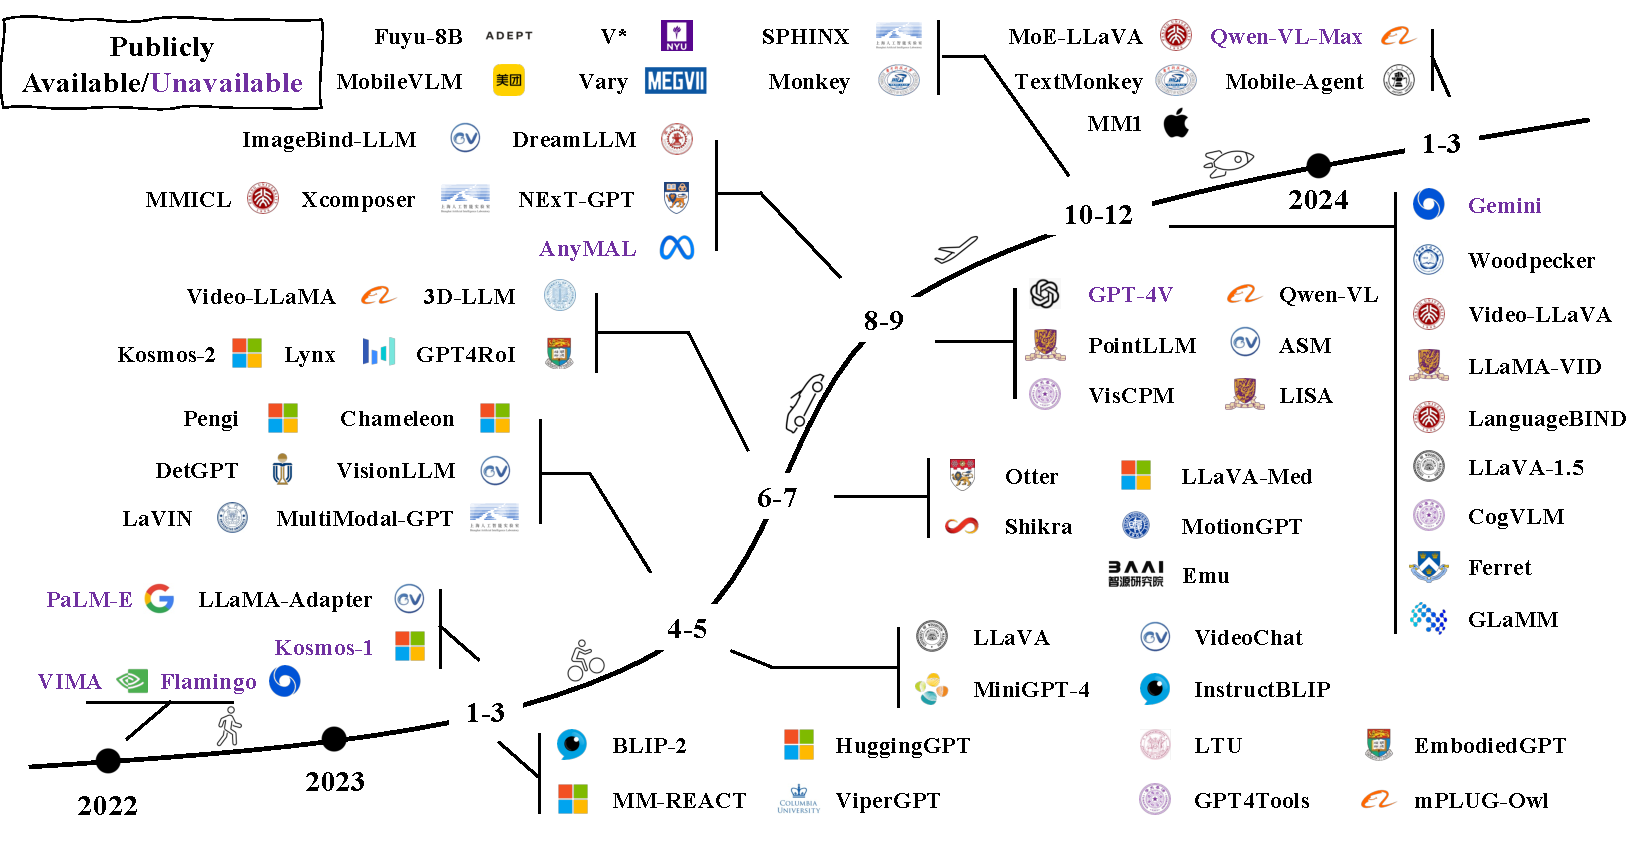
\includegraphics[width=\linewidth]{figs/survey-timeline.pdf}
    \caption{A timeline of representative MLLMs. We are witnessing rapid growth in this field. More works can be found in our released GitHub page, which is updated daily.}
    \label{fig:timeline}
\end{figure*}

Ever since the release of GPT-4~\cite{openai2023gpt4}, there has been a research frenzy over MLLMs because of the amazing multimodal examples it shows. 
Rapid development is fueled by efforts from both academia and industry. 
Preliminary research on MLLMs focuses on text content generation grounded in text prompts and image~\cite{llava,awadalla2023openflamingo}/video~\cite{videochat,video-llama}/audio~\cite{deshmukh2024pengi}.
Subsequent works have expanded the capabilities or the usage scenarios, including: 
(1) Better granularity support. Finer control on user prompts is developed to support specific regions through boxes~\cite{chen2023shikra} or a certain object through a click~\cite{yuan2023osprey}. 
(2) Enhanced support on input and output modalities~\cite{han2023imagebind, moon2023anymal}, such as image, video, audio, and point cloud. 
Besides input, projects like NExT-GPT~\cite{wu2023next} further support output in different modalities. 
(3) Improved language support. Efforts have been made to extend the success of MLLMs to other languages (\eg Chinese) with relatively limited training corpus~\cite{hu2023large, bai2023qwen}. 
(4) Extension to more realms and usage scenarios. Some studies transfer the strong capabilities of MLLMs to other domains such as medical image understanding~\cite{llava-med,moor2023med,pmc-vqa} and document parsing~\cite{ye2023mplug,liu2024textmonkey,hu2023mplug}. Moreover, multimodal agents are developed to assist in real-world interaction, \eg embodied agents~\cite{huang2023embodied,peng2023kosmos} and GUI agents~\cite{yang2023appagent,hong2023cogagent, wang2024mobile}. An MLLM timeline is illustrated in~\cref{fig:timeline}.

In view of such rapid progress and the promising results of this field, we write this survey to provide researchers with a grasp of the basic idea, main method, and current progress of MLLMs. Note that we mainly focus on visual and language modalities, but also include works involving other modalities like video and audio. 
Specifically, we cover the most important aspects of MLLMs with corresponding summaries and open a GitHub page that would be updated in real time. 
To the best of our knowledge, this is the first survey on MLLM.





